%%%%%%%%%%%%%%%%%%%%%%%%%%%%%%%%%%%%%%%%%per fare le conclusioni
\chapter*{Conclusioni}
%%%%%%%%%%%%%%%%%%%%%%%%%%%%%%%%%%%%%%%%%imposta l'intestazione di pagina
\rhead[\fancyplain{}{\bfseries
Conclusioni}]{\fancyplain{}{\bfseries\thepage}}
\lhead[\fancyplain{}{\bfseries\thepage}]{\fancyplain{}{\bfseries
Conclusioni}}
\addcontentsline{toc}{chapter}{Conclusioni}

Lo stato dell'arte al momento in cui si scrive \`e un'applicazione in grado di gestire eventi, commissioni da svolgere, spese condivise e chat, attraverso l'utilizzo di un database aggiornato e consultabile in tempo reale, e la possibilità di gestire e creare le notifiche non appena avviene un cambiamento su di esso.\\
L'applicazione pur garantendo l'uso quotidiano delle funzionalità può essere ulteriormente migliorata, aggiungendo funzionalità, rendendola più stabile e riscriverla anche per la piattaforma iOS. Alcune idee in fase di sviluppo che verrano implementante sono le seguenti:
\begin{itemize}
  \item Chat di messaggistica istantanea anche fra i singoli componenti del gruppo
  \item Migliore flessibilità e funzionalità nella gestione degli eventi
  \item Nuovi informazioni inseribili all'interno di una spesa o commissione
  \item Permettere all'untente di partecipare a più di un gruppo contemporaneamente
  \item Scrivere l'applicazione per iOS utilizzando il linguaggio Swift
\end{itemize}
Attualmente il codice dell'applicazione è presente su Gitlab\footnote{http://gitlab.com/}, in una repository privata, non appena l'applicazione sarà considerata stabile e con le funzionalità desiderate, verrà resa pubblica.\\
L'applicazione è stata scritta utilizzando il linguaggio di programmazione Kotlin, a differenza del linguaggio Java solitamente utilizzato nello sviluppo di applicazioni mobili Android.\\ L'utilizzo di Kotlin come linguaggio per lo sviluppo dell'applicazione mi ha permesso di documentarmi sui nuovi concetti introdotti dal linguaggio e porlo a confronto con Java.\\
I risultati ricavabili dal confronto effettuato, sono stati significativi soprattutto per quanto riguarda le linee di codice, infatti prendendo in considerazione una parte del progetto scritta in Kotlin e confrontato con la relativa parte del progetto precedentemente scritta in Java, alcuni file che in Java richiedevono 140 linee di codice in Kotlin la stessa logica venica implementata in circa 80 linee per quanto.

riguarda le prestazioni e la memoria utilizzata invece si hanno valori trascurabili.\\



\begin{figure}[!hb]
  \centering
  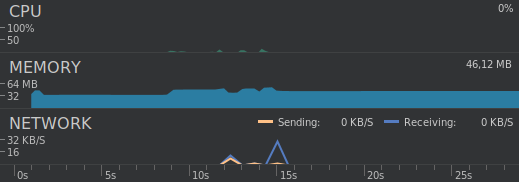
\includegraphics[width=0.8\textwidth]{immagini/app_java_memory_graph.png}
  \caption{Server Architettura}\label{fig:Android Studio }
\end{figure}

\begin{figure}[!hb]
  \centering
  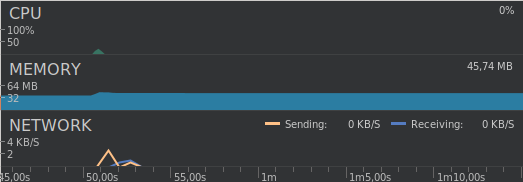
\includegraphics[width=0.8\textwidth]{immagini/app_kotlin_memory_graph.png}
  \caption{Server Architettura}\label{fig:Android Studio }
\end{figure}





\clearpage{\pagestyle{empty}\cleardoublepage}
